
\section{INTRODUCTION}
\label{sec:introduction}
% Clarify the study motivation at a high level from two points, to fit dynamical working environment and to improve human-robot-collaborations
% TO DO: mention here a clear definition of risk
Work-related low-back disorders (WLBDs) still represent a societal challenge that 
%to the current and future society,  a significant and increasing %problem that poses a 
threat the health conditions of working adults~\cite{Health1981}. Among the large variety of their causes, 
%Recent studies have shown that such kind of musculoskeletal %diseases are often caused by 
payload lifting tasks in industrial environments play a pivotal role in determining poor ergonomic conditions that favor WLBDs \cite{Kuijer2014, Lu2014, Waters2011}. In this context, ergonomics techniques to assess the quality of work conditions emerged, albeit based on qualitative questioners that are often costly and inconvenient to apply 
%Traditional pen-and-paper  are mainly based on manual observations, which can be 
for dynamically changing work environments. It is then essential to develop quantitative scalable systems that online monitor human ergonomics and that potentially alert the worker before endangering health conditions.  
%such that the user is aware of potential risks during a lifting task. Moreover, in the light of human-robot-collaborative lifting \cite{Rapetti2021}, observing human ergonomics and knowing potential lifting risks in advance are also beneficial for adjusting robot control strategies and providing efficient real-time feedback. 
This paper proposes a framework that combines wearable sensors and haptic devices, learning-based prediction algorithms and traditional lifting ergonomics to enable early assessment and active prevention of worker biomechanical risk during lifting task execution. 
% The haptic actuator integrated inside the wearables provides vibrotactile feedback to ensure the safety awareness of the worker.
%predict human and prevent  the effectiveness of continuous online assessment of human lifting ergonomics through risk prediction and haptic feedback.
%-- see Figure \ref{fig:general_framework}.
\begin{figure}[H]
    \centering
    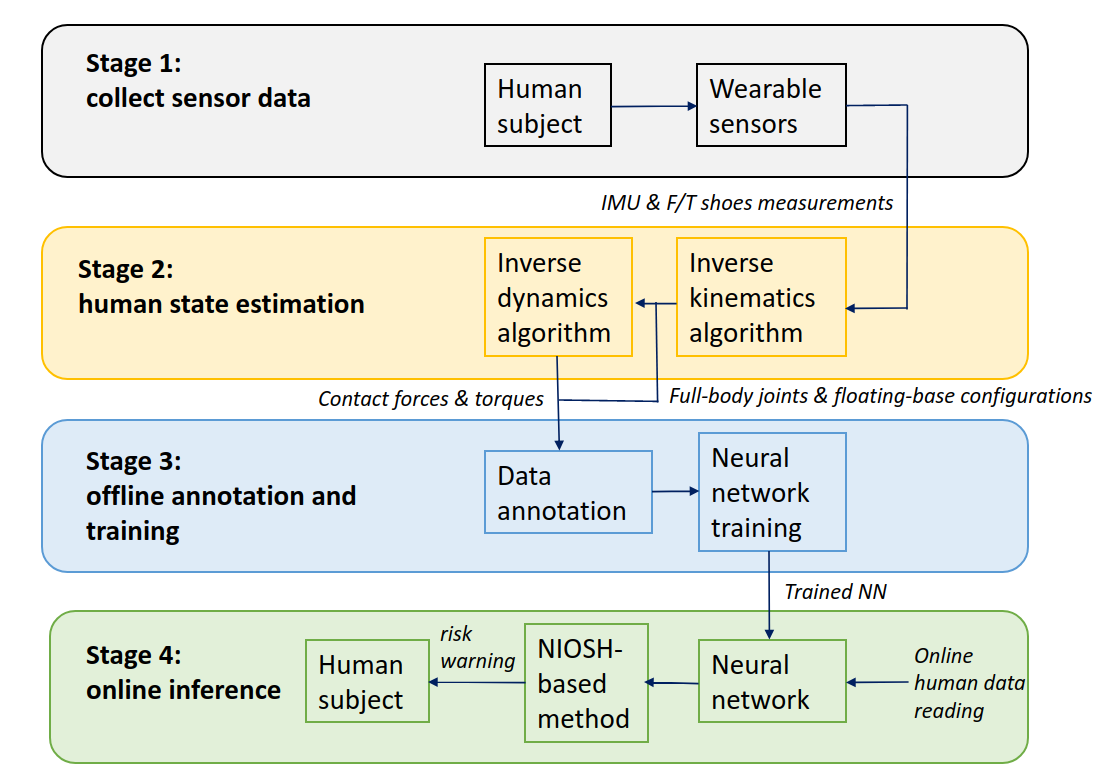
\includegraphics[scale=0.21]{figures/fig_4stages.png}
    \caption{An overview of the proposed framework.}
    \label{fig:general_framework}
\end{figure}

% Start with traditional pen-and-paper methods and some other alternatives
The \emph{Revised NIOSH Lifting Equation} (RNLE) is a renowned 
%widely used 
tool for assessing two-handed manual lifting ergonomics -- it is published by the National Institute for Occupational Safety and Health (NIOSH) \cite{Waters1993, Waters1994}. The RNLE defines a \emph{Recommended Weight Limit} (RWL) and a \emph{Lifting Index} (LI) based on payload weight, which may lead to reliable risk assessment for  
%The LI has been proved to be valid for indicating risks of 
WLMDs \cite{Waters2011}. Unfortunately, approximately 35$\%$ of lifting tasks and 63$\%$ of workers can not be assessed by means of the RNLE due to its limited number of parameters and system constraints \cite{Dempsey2002}. To overcome such limitations, further approaches have been proposed to assess lifting-related risks, e.g., \emph{L5-S1 Internal Forces} \cite{Lavender2003}, \emph{Mechanical Energy Consumption} \cite{Ranavolo2017} and \emph{Muscles Co-Activation} \cite{Ranavolo2015}. However, these offline ergonomics evaluation tools are not flexible enough to be used directly in an unstructured work environment. 

As an attempt towards online human ergonomics evaluation, observational methods -- like the \emph{Rapid Entire Body Assessment (REBA)} and \emph{Rapid Upper Limb Assessment (RULA)} -- are leveraged for human-robot interaction \cite{Shafti2019}.
%and \cite{} exploit the  by integrating them into a human-robot-interaction system. 
The human data are measured by wearable sensors and an estimation of motion's ergonomics is provided by automatically fulfilling the worksheet. More recently, real-time tools for tracking joint compressive forces during robot interactions are employed \cite{Fortini2020ROMAN}. 
%This tool monitors human ergonomics by assessing joint risks introduced by external physical interactions with robots. 
Analogously, the overloading joint torques can be computed using the displacement of the center of pressure during heavy lifting tasks, returning visual feedback of the worker state \cite{fortini2020framework}.
%of ergonomics status is illustrated to the human subject The authors also proposed another framework for online ergonomics monitoring in , where . 
%In these approaches, which overcome environment restrictions and privacy constraints of vision-based techniques, risk prediction is still missing.
%This work shows that IMU-based monitoring system outperforms  who suffer from space restrictions and privacy problems.
%
% From literature to our work
%The studies above demonstrate the possibility of integrating observational ergonomics tools with advanced sensing systems and motion-tracking methods for online evaluation and monitoring of human ergonomics. But 
For manual lifting tasks, the existing attempts are either overly generic, e.g.  \cite{Shafti2019}, or limited by hardware settings, e.g. portability restriction \cite{fortini2020framework}. They also lack the ability to alert the worker in advance, beforehand that biomechanical risks endanger health conditions. 
% THIS IS A CONTRIBUTION Hence we propose a framework that combines the commonly-used RNLE tool with some of our previous work (e.g., wearable sensing suits, human state estimation \cite{Rapetti2020}, human action and motion prediction \cite{Kourosh2022}) to fill the gap between offline and online human lifting ergonomics monitoring models. 

%In context of this research, IMU-based sensing system has more advantages over vision-based approaches when used for human motion tracking, not only due to an easier calibration but also more convenient application in a wider space. According to \cite{Von2017, huang2018deep}, with only 6 Inertial Measurement Units (IMUs), the \emph{state-of-the-art} is capable to reconstruct human full-body pose in real-time. In comparison, our sensing suit requires 10 IMUs and a pair of Force/Torque shoes only considering essential human links. The IMUs measurements are used for human kinematics and dynamics estimation. Assuming human skeleton is modeled as a multi-rigid-body system, the state estimation can be solved as \emph{Inverse Kinematics} and \emph{Inverse Dynamics} problems. Various approaches can be found in literature for solving them, e.g., analytic solution \cite{Tan2019, Ancans2021}, instantaneous optimization \cite{Kok2014, Von2017}, dynamical optimization \cite{Andrews2016, Suleiman2018}, learning algorithms \cite{Grochow2004} and etc. 
Generally, human action recognition and motion prediction are tackled as two separate issues.
Action recognition can be addressed as a classification problem, solved by applying supervised learning methods \cite{Zhao2019, Ji2012}. Motion prediction is more often regarded as a regression problem, that has been addressed for example by means of generative adversarial networks \cite{Hernandez2019}, graph convolutional networks \cite{Mao2019}, dropout auto-encoder LSTM \cite{Ghosh2017}. 
In \cite{Kourosh2022}, it was proposed the \emph{Guided Mixture of Experts} (GMoE) framework that can resolve these two problems simultaneously, having the potential to simplify the architecture for motion prediction and risk assessment.
%often simplifying the overal learning architecture for risk assessment and which can be further adopted in this case.

% paper main contributions
This paper proposes a learning-based approach that enables predictions of worker biomechanical risk during lifting tasks with anticipated haptic feedback. We use IMU-based sensing systems that show some advantages over vision-based approaches when used for human motion tracking due to easier calibration and a more convenient application in wider, partially occluded spaces. Moreover, the wearable device can integrate the actuation unit to provide feedback to the subject.
%According to \cite{Von2017, huang2018deep}, with only 6 Inertial Measurement Units (IMUs), the \emph{state-of-the-art} is capable to reconstruct human full-body pose in real-time. In comparison, 
The employed wearable system is composed of 10 IMUs with haptic actuators and a pair of Force/Torque shoes.
%from which 
%considering essential human links. The IMUs measurements are used for human kinematics and dynamics estimation. Assuming human skeleton is modeled as a multi-rigid-body system, the
% state estimation can be solved as \emph{Inverse Kinematics} and \emph{Inverse Dynamics} problems. 
%Various approaches can be found in literature for solving them, e.g., analytic solution \cite{Tan2019, Ancans2021}, instantaneous optimization \cite{Kok2014, Von2017}, dynamical optimization \cite{Andrews2016, Suleiman2018}, learning algorithms \cite{Grochow2004} and etc.  
The contribution of this paper is threefold. First, we develop a system that can monitor human ergonomics online in the context of lifting activities. To do so, we propose a framework that integrates both the human state estimation algorithm and human action/motion prediction method, enabling the RNLE to not only estimate but also predict lifting risk continuously. Second, we adapted the GMoE \cite{Kourosh2022} approach for recognizing a set of predefined actions that compose a complete lifting activity. The GMoE network is trained on a data set collected in a laboratory environment. Finally, we validate online the proposed framework via an experimental analysis conducted on lifting tasks.

% paper content organization
The paper is organized as follows. In Section \ref{sec:background} we introduce the underlying technologies used in our research. In Section \ref{sec:methods} the proposed framework is clarified, including the implementation of RNLE-based human lifting ergonomics monitoring system. Section \ref{sec:validation} presents an experimental analysis conducted on a human subject. At last, Section \ref{sec:conclusions} concludes the paper.